%\RequirePackage[2020-02-02]{latexrelease}
\documentclass[12pt]{article}
%\documentclass[lineno]{biometrika}

%% packages
\usepackage{star}
\usepackage{tikzit}
\input{tikz/sample.tikzstyles}
\usepackage{natbib}
\usepackage{circuitikz}
\usepackage[toc,page]{appendix}
\def\ride{{\overrightarrow{s}}}
%% Please use the following statements for
%% managing the text and math fonts for your papers:
\usepackage{rotating}
\graphicspath{{img/}{tikz/}{img/tikz/}}

\usepackage[a4paper,
            bindingoffset=0.2in,
            left=0.5in,
            right=1in,
            top=0.75in,
            bottom=0.75in,
            footskip=.25in]{geometry}

\providecommand{\keywords}[1]{\textbf{\textit{Keywords ---}} #1}


%%%%Main Document
\begin{document}

\title{On pricing of rides on transportation networks}

\author{Mohamad Elmasri\thanks{Department of Mathematics and Statistics, Carleton University\texttt{mohamadelmasri@cunet.carleton.ca}.}}
\date{\today}
\maketitle
\tableofcontents

\vspace{-0.25in}
\begin{abstract}
    This work addresses the challenge of pricing complex transportation products in modern ride-sharing markets, where rides are priced in advance under travel time uncertainty.  Focusing on the problem of pricing commuter memberships with a capped maximum cost, we propose a novel approach that leverages financial tools and recent advances in travel time distribution modeling.  By characterizing the distribution of ride prices on a transportation network represented as a metric graph with a cyclostationary travel time process, we derive an analytical solution for upfront pricing that guarantees a predetermined ride price. This framework allows for both population-level and trip-specific pricing strategies.  Our findings contribute to a deeper understanding of pricing mechanisms in transportation networks and offer practical solutions for designing innovative commuter benefits.
\end{abstract}
\section{Introduction}
\subsection{Background}
Mobility is vital to human activities, forming an integral component of our economic and trade networks, social interactions, political ties, and overall quality of life. Large-scale, trip-level data with extensive temporal and spatial coverage enables us to better diagnose transportation problems and develop effective solutions. Classical taxi providers priced rides based on actual time and distance traveled, with payment upon arrival. In contrast, modern ride-sharing services\footnote{Such as, Waymo Inc., Lyft Inc., and Uber Inc.} are required to price rides well in advance. Commuter rides, for example, are priced a month, if not a year, in advance. However, pricing more complex products, such as the right to travel a route for a predetermined fixed price, remains a challenge.

Two immediate challenges exist to achieve a general approach to pricing rides in transportations networks: 
understanding price variability in the marketplace and developing a modular, easily computable framework for pricing complex products. Price variability is predominantly influenced by travel uncertainty and supply and demand dynamics, the latter often controlled by ensuring sufficient driver availability. Recent progress in understanding travel uncertainty has demonstrated, both theoretically and in practical applications, that long-term deviations in travel time behave similarly to deviations from a normal distribution, despite the apparent chaotic nature of real-world traffic~\cite{elmasri2020predictive, woodard2017predicting}.

This work redefines the ride-sharing pricing problem as the pricing of contractual agreements for specified deliveries, where future transportation services are provided for a predetermined price. Building on the work of~\cite{elmasri2020predictive}, we price these agreements using well-established financial tools, providing a novel method to price complex transportation products, including, but not limited to, those mentioned earlier. We focus on strategically designing transportation incentives that transform the commuter experience by offering financial guarantees that reduce pricing uncertainty\footnote{Consider a business establishment Such as, a gym, medical clinic, or a work office. with repeating clients, frequenting on a specific timeline. To establish a stronger business-client relation, the business is considering providing personalized transportation packages, where clients have the option to cap their trip cost to a predetermined amount, regardless of the actual cost.}. In particular, we are interested in giving a definite answer to the following question:
\begin{quote}
    How to price a commuter membership that ensures a maximum trip cost of K\$?
\end{quote}


\subsection{Motivating toy example}
To motivate an answer to the above question, we provide some intuition on the distribution of pricing that is partially observed in rides-share market in a simulated toy example. Consider the assumption a ride request is always fulfilled on route $\path$ (sufficient supply of liquidity). Assume that rides do not interfere with each other. Let $P_\path(t)$ be of such ride at start time $t>0$. Varying the start time constitutes, hypothetically, a continuous stream of rides across $\path$, and henceforth a realization of a continuous pricing function. Repeating this many times results in a continuous distribution of price over $\path$. 

We show five realization of such distribution (Fig.~\ref{fig:true-price}) by dividing a 24-hour period into 1-minute intervals. For each minute, a ride was simulated on a fixed route consisting of 100 edges, each 100 meters in length. To simulate varying traffic conditions, the speed of each edge in every ride was sampled from a log-normal mixture model with two states: non-congested and congested, as described in~\citep{woodard2017predicting,guo2012multistate, elmasri2020predictive}. The non-congested state, occurring with a probability of 0.8, had a mean speed of 35 km/h and a standard deviation of 5 km/h, sampled as logNormal\((\mu=\ln(35),\sigma=\ln(5))\). The congested state had a mean speed of 5 km/h and a standard deviation of 10 km/h.

To simulate rush hour conditions, the probability of congestion was increased to 0.8 between 7:00 and 9:00 and again between 16:00 and 18:00. The round circles, in Figure~\ref{fig:true-price}, are actual realizations of prices observed over time. In that sense, the pricing distribution is only partially observed. 
\begin{figure}
    \centering
    
\includegraphics[width=0.8\textwidth]{img/price.jpeg}
    \caption{True price for rides starting at time $t$ over a fixed path $\path$. The price line is represent hypothetical rides, except at circled dots.}
    \label{fig:true-price}
\end{figure}



\subsection{Outline}
We start with the necessary background material (Sec.~\ref{sec:background}), where we introduce the concept of metric graphs (Sec.~\ref{sec:metric-graph}) and cyclostationary processes on such graphs (Sec.~\ref{sec:cyclostationary}). With such info, we define the travel time process (Sec.~\ref{sec:traveltime-process}). Section~\ref{sec:pricing-main} establishes our first objective of characterizing the pricing equation in ride-share markets, its distribution, and the necessary assumptions to achieve our result. We solve, in Section~\ref{sec:upfront}, an analytical equation for up-front pricing of on-demand (instantaneous rides) that guarantees a fixed predetermined price. We do so for population and trip-specific rides, building on the work~\cite{elmasri2020predictive, woodard2017predicting} and establishing our second objective. Finally, we develop a more comprehensive framework for pricing complex transportation products, such as commuter rides, in Section~\ref{sec:complex-pricing}. We demonstrate our work in a case study in Section~\ref{sec:case-study}.

\subsection{Literature review}

Previous research has shown that incorporating uncertainty into travel time estimates can lead to improved outcomes in ride-sharing systems, such as higher driver-rider match rates (up to 85\%) and lower average prices (up to 12\%) \citep{long2018ride}. These improvements can also positively impact other key system metrics, including reliability, service rate, utilization, and profitability \citep{li2021vehicle, li2022pricing,li2022ride}. Consequently, interest in understanding travel time uncertainty has been growing for practical reasons \citep{westgate2013travel,wang2019simple, hunter2009path,westgate2016large}.  Researchers have explored various approaches, ranging from models that estimate uncertainty from individual edges \citep{zheng2013urban,jenelius2013travel} to those that estimate route and travel uncertainty simultaneously \citep{westgate2013travel,wang2019simple, hunter2009path,westgate2016large}. With the increasing volume of collected GPS data, research has primarily focused on understanding the distribution of travel time through parametric methods \citep{woodard2017predicting,guo2012multistate,ma2017estimation,zhang2019novel} or by examining the limiting properties of stochastic and dynamical processes resembling real-world travel behavior \cite{elmasri2020predictive, bolin2022gaussian}.

Recent progress has shown that deviations in travel time behave similarly to deviations from a normal distribution~\cite{elmasri2020predictive, woodard2017predicting}. Therefore, it is not surprising that regression-based models have shown promising results in travel time modelling \citep{westgate2016large, woodard2017predicting,budge2010empirical, westgate2013travel}. In particular,~\cite{elmasri2020predictive} have suggested a Gaussian form as a population-style distribution for travel time, where both the mean and variance scale with distance. For example, a \(N(n\mu, n\sigma^{2})\), where \(n\) is the number of road segments and \((\mu, \sigma^{2})\) are map- (possibly traffic time bin-) specific mean and variance constants. A similar distribution has been proposed for route-conditional travel time. 


For a survey of dynamical processes on networks (including transportation networks), see~\citet[ch. 11]{barrat2008dynamical}, for resent statistical work on the topic see~\citep{kolaczyk2014statistical, snijders2017modeling,burk2007beyond, britton2002bayesian,golightly2005bayesian, bolin2022gaussian}. 

[need to add literature review on pricing]

\section{Background}\label{sec:background}
\subsection{Metric graphs}\label{sec:metric-graph}
A finite graph $\cG = (\cV, \cE)$ consists of a set of a finite set of vertices $\cV =\cbr{v_i}$ and a set $\cE = \cbr{e_j}$ of edges connecting the vertices. We write $u \sim v$ or $\rbr{u,v} \in E$  if $u$ and $v$ are connected with an with edge. We let $\cG$ be a direct graph, that is, $\rbr{u,v}$ represents and edge from $u$ to $v$. We call a graph $\cG$ a metric graph, if every edge $e$ is assigned a length $0< l_e< \infty$, and over $e$ it possible to assign a coordinate  $c \in [0, l_e]$ which increases in a specified (but otherwise arbitrary) direction along the edge. Since the length $l_e$ are assumed to be finite, this implies that the graph is compact. A point $s \in \cG$ is a position on an edge, i.e.~$s = (e, x)$, where $x \in [0, l_e]$. A path $\path = \pathseq{\pstart}{\pend} \in \cG$ is a sequence of edges $\rbr{e_1, \dots, e_n}$ where the path starts at point $\pstart \in e_1$ and ends at $\pend \in e_n$. A natural choice of metric for the graph is the shortest path distance, which for any two points in $\cG$, it is defined as the length of the shortest path in $\cG$ connecting the two. We denote this metric by $\delta(\cdot, \cdot)$ from now on. We provide a path conditional version of this distance metric as $\delta_\path(s) = \delta_\path(s, \pstart)$, for $s \in \path$, as the distance between points $s$ and the start of the path $\pstart$, over the the path. We further let $\delta_\path$ defines the whole distance of $\path$. Let $n_\path = \abr{\cbr{e : e \in \path}}$ be the number of edges of $\path$. We assume that the graph is connected, so that there is a path between all vertices. We define $\Pi(e_1, e_2)$ to be the set of all paths between edge $e_1$ and $e_2$, and for every two edges $e_1, e_2 \in \cE$, let $\pi(e_1, e_2)$ be the probability that a ride starts at $e_1$ and ends at $e_2$. Here, we have modelled the joint dis

There is no unique way of defining process over graphs. This is a result of various way of defining the boundary condition (vertex condition), such as the Neumann-Kirchhoff condition, see~\citet[Eq~(1.4.4) and Them~1.4.4]{berkolaiko2013introduction}. In this work, we treat a path $\path = \pathseq{\pstart, e_1}{e_n,\pend}$, as an extended sequence of an uninterpreted edge, having the geometry
\[\sbr{0,\;  \delta(\pstart, e_1) + \sum_{e\in \path} l_e + \delta(e_n, \pend)}, \]
without introducing intermediate vertices at $l_e,$ $e \in \path$.


For every edge $e\in \cE$, a function $f_e \in L_2(e)$ if $f_e$ is square-intergrable over the edge $e$. We further define a function $f$ over $\cG$ as a collection of functions $f = \cbr{f_e}_{e \in cE} \in L_2(\cG)$ if $f_e \in L_2(e)$ for each $e \in \cE$. Tihs results in $L_2(\cG)$ being the direct sum over $L_2(e)$ as 
\[L_2(\cG) = \bigoplus_{e \in \cE} L_2(e). \]

We finally let $C(\cG) = \cbr{f \in L_2(\cG): f \text{ is continuous}}$ be the space of continuous functions on $\cG$. We define $\RR_+$ to be the postitive part of the real line.

\subsection{Cyclostationary processes over metric graphs}\label{sec:cyclostationary}
We let $X=X(t, s)$, for every fixed time index $t \in \RR_+$ and point $s \in \cG$, be a 2nd order cyclostationary process in the wide sense. Here $X(t,s)$ is spatio-temporal process defined as
\begin{equation} \label{eq:speed}
X(t,s) = m(t, s) + \epsilon(t, s), \qquad t \in \RR_+, s \in \cG,
\end{equation}
where, in the temporal domain (holding the spatial fixed), for every $e \in \cE$ and $t, u \in \RR_+$, we have
\begin{subequations}
\label{eq:mean-covariance}
\begin{align}
    m(t, s) & =\EE[X(t,s)] = m(t + T_e, s), \label{eq:mean}\\
    \sigma^2(t, s) &= \EE[\epsilon^2(t,s)] = \sigma^2(t +T_e, s), \label{eq:variance}\\
    \varsigma(t, u, s) &= \EE[\epsilon(t,s)\epsilon(u, s)] = \varsigma(t +T_e, u+T_e, s) \label{eq:covariance},
\end{align}
\end{subequations}
where $T_e \in \RR_+$ is an absolute positive constant defining the temporal cycle of edge $e$. Here, $m(t,s), \sigma^2(t,s), \varsigma(t,u, s) \in C(\cG)$ (measurable functions over $\cG)$, and $\EE[\epsilon(t,s)]=0$ for all pairs $(t, s) \in \RR_+ \times \cG$.  We further let $\max_{e\in \cE} T_e \leq T_\cG < \infty$ be the global temporal cycle over $\cG$. That is, all equalities in~\eqref{eq:mean-covariance} apply when replacing $T_e$ by $T_\cG$. By definition of cyclostationarity, for come absolute constant $U_1>0$, we have
\[\abr{m(t,s)} + \abr{\sigma^2(t,s)} \leq \max_{u \in [0, T_\cG]}\cbr{m(u, s), \sigma^2(u, s)} \leq U_1,\]
for all $t\in \RR_+$, which is a stronger condition than the classical growth condition imposed on stochastic random variables, see~\citet[Thm.~5.2.1]{oksendal2013stochastic}. We further assume Lipschitz continuity in space and time as 
\begin{equation}\label{eq:lip-condition}
    \abr{m(t,x) - m(u, y)} + \abr{\sigma^2(t,x) - \sigma^2(u,y)} \leq C_2 \cbr{\abr{t-u} + \abr{x-y}},
\end{equation}
for $t, u \in \sbr{0, T_\cG}$, $x,y \in \cG$, and $C_2>0$ is an absolute constant.~\eqref{eq:lip-condition} results in spatial Lipschitz continuity when $t=u$, and temporal when $x=y$. 

We assume a conditional independence condition between space and time, that is is 
\[X(t, x) \perp X(t, y) \;\given\; t; \qquad x,y \in \cG, x\neq y.\] 

We define a ride on $\cG$ to be a the pair $(\rho, t)$, representing the path $\rho$ of the ride and the start time $t>0$.

%We further define the space of temporal marginal random variables as 
% \begin{equation}\label{eq:maringal-speed}
%     X_e(t) = \int_{s\in e} dX(t,s), \quad \text{for } e % \in E
% \end{equation}
% with temporal marginal mean and variance functions as 
%\[m_e(t) = \int_{s\in e} m_e(t, s)ds\qquad \sigma^2_e(t) = \int_{s\in e} \sigma^2(t,s)ds,\]
% where we equip $m_e$ and $\sigma_e$ with the subscript that indicates the marginal for edge $e$. %The spatial marginal mean and variance functions are \[m(s) = \int_{(0, C_s]} m_e(t, s)dt\qquad \tau^2(s) = \int_{(0, C_s]} \sigma^2(t,s)dt,\]
%where $C_s$ is the temporal length of the cycle at point $s$. 



% A sequence of random variables that exhibit such a form of serial dependency, 
% with variables far apart being nearly independent, is referred to as a {\it mixing } sequence. Different mixing types have been introduced in the literature. Each mixing type is associated with a separate coefficient assessing its strength~\citep{bradley2005}. The most general, in a sense implied by many other types, is called \(\alpha\){\it -mixing} (strongly mixing), which is defined below.

% \begin{definition}[\citep{rosenblatt1956central}] \label{def:alpha-mixing} Let $(X_k, k \in \Z)$ be a sequence of random variables defined on the probability space $(\Omega, \F, P)$. Define the $\sigma$-algebra $\F_a^b$ as
% \(\F_a^b = \sigma(X_k, a\leq k \leq b, k \in \Z)\), \(1 \leq a \leq b\leq \infty.\)
% For each $n\geq1$ define the measure of dependence
% \begin{equation}\label{eq:alpha-mixing}
%     \alpha(n)= \sup_{k \geq 1}\sup_{A \in \F_1^k, B \in \F_{k+n}^\infty} |P(A \cap B) - P(A)P(B)|.
% \end{equation}
% If $\alpha(n) \rightarrow 0$ as $n\rightarrow \infty$, then $(X_k, k \in \Z)$ is said to be {\it $\alpha$-mixing}.
% \end{definition}

% Since \(X(t,s)\), for\(t>0, s \in \RR^2\), are not strictly stationary (meaning that they do not have a time-invariant distribution), we require an extra mixing condition that is slightly stronger than the maximal correlation coefficient (defined as \(\rho(n)\) in \cite{bradley2005}) and implies it, which is related to mixing of interlaced sets.
% \begin{definition} \label{def:rho-mixing} Following 
% Definition 
% \ref{def:alpha-mixing}, let \(\F_{A} =\sigma(X_{i}, i \in A)\) for any non-empty set \(A \subset \Z\). Define the dependency measure
% \begin{equation}
%   \label{eq:rho-mixing}
%   \trho (n)= \sup_{A, B}\sup_{f,g} |\Corr(f,g)|, \quad  f \in \L^{2}(\F_{A}),\; g \in \L^{2}(\F_{B}), \min_{i\in A,j\in B }|i-j| \geq n,
% \end{equation}
% where \(\L^{2}(\F_{A})\) denotes the space of square-integrable \(\F_{A}\) random variables, and the supremum is over all disjoint non-empty sets \(A, B \in \Z\).
% \end{definition}
\subsection{Travel time process}\label{sec:traveltime-process}
We first define a transportation network $\cN = (\cG, X)$ to be a metric graph $\cG$ equipped with wide-sense cyclostationary process $X(t, s)$, $t \in \RR_+$ and $s \in \cG$. Travel time over a path $\path = \pathseq{\pstart}{\pend} \in \cG$ can be directly computed as the stochastic integral 
\begin{equation}
    \label{eq:traveltime-process}
\T_\path = \int_\path X(\T_s, s)ds = \int_\path m(\T_s, s)ds + \int_{\path} \epsilon(\T_s,s)ds, \quad \T_\pstart = 0
\end{equation}
where $\int_\path$ represent integration over the predetermined path $\path$, with $s \in \path$ being a point over the path. Here, $T_s, s \in \path$ defines the travel time up to location $s$ on $\path$, such that the travel time at the start point $\pstart$, $\T_\pstart =0$. ~\cite{elmasri2020predictive} approximated the integral~\eqref{eq:traveltime-process} by a discrete version $\T_\path^d$, as 
\[\T^d_\path = \sum_{e \in \path} m_e(\tau_e) + \epsilon_e(\tau_e), \]
where 
\begin{equation}\label{eq:marginals}
    m_e(t) = \int_e m(t,s)ds, \quad \sigma^2_e(t) = \int_e \sigma^2(t,s)ds, \quad \epsilon_e(t) = \int_e \epsilon(t,s)ds,
\end{equation}
for $t \in \RR_+$.~\eqref{eq:marginals} are the spatial marginals over $X(t,s)$ defined in~\eqref{eq:speed}. Here, $\tau_e$ is the random arrival time at edge $e$. We have implicitly assumed that all edges are traversed in $\T_\path^d$, and that $\T_\path^d$ is defined on a transportation network $\cN^d$ defined by the marginals of $X$, such that $\cN^d = (\cG, X^d)$, and $X^d = \cbr{X_e(t)}_{e \in \cE}$, where $X_e(t) = \int_e X(t,s)ds$. The following lemma is an adaptation of \citet[Lem~6, Them.~6]{elmasri2020predictive} that characterize the asymptotic distribution of $\T_\path^d$. 

\begin{lemma}[Population distribution~\cite{elmasri2020predictive}] \label{lem:population-distribution}Consider $\path$ as a random walk over the $\cN^d$ and let $\tau = \cbr{\tau_e}_{e \in \path}$ be the random arrival times over edges of the walk $\path$. Let  $\tau$ be sufficiently mixing\footnote{at least $\rho$-mixing, see~\cite{bradley2005} and \citet[Lem.~5,6]{elmasri2020predictive}}. Then as the number of edges in $\path$ grow to infinity (i.e.~$n_\path \to \infty)$, we have
\begin{subequations}\label{eq:population-asymp-dist}
\begin{align}
    n_\path^{-1}\T^d_\path &\stackrel{\text{a.s.}}{\to} \mu \\
    n_\path^{-1/2}(\T^d_\path - n_\path\mu) &\stackrel{d}{\to} N(0,\sigma^2), \label{eq:population-distribution}
\end{align}
\end{subequations}
where $\mu$ and $\sigma^2$ are absolute positive constants that are independent of initial conditions and of $\path$. 
\end{lemma}

The result in~\eqref{eq:population-asymp-dist} suggest that deviations of $\T_\path$ around the average travel time per edge $\mu$, normalized by $\sqrt{n_\path}$, resemble independent samples from a normal distribution, with variance that is independent of the route. However,~\eqref{eq:population-asymp-dist} is an asymptotic distribution over a population of rides in a system. That is for an arbitrary ride from a population of rides, the probability it arrives before $n_\path\mu$ is $1/2$. For a specific ride, say $(\rho_i, t_0)$, this probability can be significantly different if $\T_{\path_i}$ has not reached the asymptotic distribution. The following lemma is an adaptation of~\citet[Thm.~7]{elmasri2020predictive} that characterized the distribution of travel time for a specific ride. First, we define a deterministic mean and covariance sequences for a ride over $\path=\pathseq{e_1}{e_{n_\path}}$, starting at $t_1\in \RR_+$, as
\begin{subequations}\label{eq:mean-covariance-seq}
    \begin{align}
        t_{i+1} &= t_{i} + m_{e_i}(t_i), \quad i \in \cbr{2,\dots, n_\path},\\
        \mu_\path &= \sum_{i =1}^{n_\path} m_{e_i}(t_i), \\
        \sigma^2_\path &= \sum_{i=1}^{n_\path} \sigma^2_{e_i}(t_i) + 2 \xi \sum_{i=2}^{n_\path}\sigma_{e_i}(t_i)\sigma_{e_{i-1}}(t_{i-1}),
    \end{align}
\end{subequations}
for some absolute constant $\xi$. Here, $m_e$ and $\sigma^2_e$ are the spatial marginals defined in~\eqref{eq:marginals}. 

\begin{lemma}[Route-predictive distribution, Thm.~6 in~\cite{elmasri2020predictive}] \label{lem:route-predictive} Under the conditions of Lemma~\ref{lem:population-distribution}, for an arbitrary start time $t_1 \in \RR_+$, given a path $\path=\pathseq{e_1}{e_{n_\path}} \in \cG$, we have 
\begin{equation}\label{eq:route-distribution}
    \sigma^{-1}_{\path} \rbr{\T^d_\path - \mu_\path} \stackrel{d}{\to} N(0, \eta), \quad \text{as  } n_\path \to \infty,
\end{equation}
where $\eta$ is a strictly positive constant that is independent from initial conditions, and $\sigma^2_\path $, $\mu_\path$ are defined in~\eqref{eq:mean-covariance-seq}. 
\end{lemma}

The result of Lemma~\ref{lem:route-predictive}, although still suggests approximate normality of travel time distribution, it integrates route-specific information in the mean and covariance functions~\eqref{eq:mean-covariance-seq} to better approximate this distribution. As shown in~\citet[Fig.~3]{elmasri2020predictive}, the approximation in~\eqref{eq:route-distribution} can achieve significant accuracy when compared to~\eqref{eq:population-distribution}. 

Working with $\T_\path$ in~\eqref{eq:traveltime-process} directly is challenging, since the distribution of $\epsilon$ is not well understood. Every edge $e \in \path$ can influence $\T_\path$ differently, depending on the cyclostationarity pattern of the variance $\sigma(t,s)$ and the actual error distribution. 

To overcome such challenges, we rely on the results in Lemma~\ref{lem:population-distribution} and~\ref{lem:route-predictive}. The mean and covariance functionals $\mu(t,s)$, $\sigma(t,s)$ in~\eqref{eq:mean-covariance} define manifolds over the graph $\cG$. Using the asymptotic normality of travel and those functionals, we redefine travel time as the stochastic process, initiated at $\pstart=0$, as
\begin{equation}\label{eq:stochastic-travel-time}
    d\T_{s} = \alpha(\T_{s}, s)ds+ \beta(\T_{s}, s)dB_s,\qquad \T_0 = 0,   \quad s \in \path,
\end{equation}
where $B_s$ is Brownian process.~\eqref{eq:stochastic-travel-time} suggests that travel time over a route $\path$ behaves like an arithmetic Brownian motion on the spatial domain, having the expectation and variance as 
\[\EE[\T_s] = \int_\path \alpha(\T_s,s)ds \quad \Var[\T_s]  = \int_\path \beta^2(\T_s, s)ds, \quad s \in \path,\]
where the variance follows by the assumption that $B^2(t,s)$ is bounded, and thus by the Itô isometry property \citet[Lem.~3.1.5]{oksendal2013stochastic}, we have $\EE\rbr{\int_\path \beta(\T_s, s)dB_s}^2 = \int_\path \beta^2(\T_s,s)ds$. 

Finally, to adapt $\T_\path$ to the population version in Lemma~\ref{lem:population-distribution} and the route-specific version in Lemma~\ref{lem:route-predictive}, we let $\alpha$ and $\beta$ be 

\begin{equation}\label{eq:mean-variance-sde}
    \alpha(t,s) = 
    \begin{cases}
        \mu & \text{population} \\
        m(t,s) & \text{route-specific}
    \end{cases}
    \qquad 
    \beta(t,s) = 
    \begin{cases}
        \sigma & \text{population}        \\
        \sqrt{\eta}\sigma(t,s) & \text{route-specific},
    \end{cases}
\end{equation}
where $m(t,s)$ and $\sigma(t,s)$ are as defined in~\eqref{eq:mean-covariance} and $\eta$ is a universal parameter that is estimated from data and accounts for residual error. 


\section{Pricing equation in ride-share markets}\label{sec:pricing-main}
Ride pricing is determined by three constant factors predefined by the service provider. A fixed price $C_0$ (starting price), a cost for a unit of time $C_1$, and a cost for a unit of distance $C_2$. Let $P_\path(s, t)$ be the price of a ride that starts at time $t>0$, over the route $\path$, and at location $s \in \path$, that is
\begin{equation}\label{eq:price}
    P_\path(s, t) = C_0 + C_1\T_s(t) + C_2 \delta_\path(s), \qquad s \in \path, 
\end{equation}
where $\T_s(t) = \T_{\path(s)}(t)$ is the travel time up to point $s \in \path$ and starting at time $t>0$ and $\delta_\path(s) = \delta(s,\pstart)$ is the length of the path $\path$ up to point $s$. To simplify notations, we will drop the $(t)$ from $\T_s(t)$, since the start time defined in the pricing function $P_\path(s, t)$. The base price is determined at the start point $\pstart \in \path$, that is 
\[P_{\pstart}(\pstart, t) = C_0, \quad \text{for all } t > 0, \]
and the final price is determined at the destination point $\pend$, and arrival time $t_0$, as
\[P_\path(\pend, t) = C_0 + C_1\rbr{t_0 - t} + C_2\delta_\path.\]

Here,  $\T_{\path(\pend)} = t_0 -t$, an actual realization. Otherwise, for any point $s \in \path \setminus \cbr{\pstart, \pend}$, the price equation~\eqref{eq:price} is a random variable determined by $\T_s(t)$. Moreover, for any two points $s_1, s_2 \in \path$, if $s_2$ is further along $\path$ than $s_2$ (i.e.~$\delta_\path(s_1) \leq \delta_\path(s_2)$), then 
\[P_\path(s_2,t) \geq P_\path(s_1,t).\]

Such inequality in the time domain is not true, that is $P_\path(s, t_1)$ is not necessary less than $P_\path(s,t_2)$ for $t_1 < t_2$, and $s \in \path$. The price equation~\eqref{eq:price} is, thus, composed of three components: (i) the fixed price $P_\path(0,0) = C_0$, (ii) the incremental price $C_2\delta_\path(s)$, and (iii) the variable price $C_1\T_s, s \in \path$. In this sense, the true price of a ride over $\rbr{t,\path}$ that arrived at $\T_\path = t_0 - t$, is 
 \begin{equation}\label{eq:true-price}
    P_\path(\pend, t) = C_0 + C_1(t_{0} -t) + C_2 \delta_\path,
 \end{equation}

 If the realization is not yet observed, then the present value of the ride price at start location $\pstart$ is a random variable having the expectation
\begin{equation}\label{eq:predicted-price}
    P_\path(\pstart, t) = \EE\sbr{P_\path(\pend, t)}= C_0 + C_1\EE\sbr{\T_\path} + C_2 \delta_\path,
 \end{equation}

In~\eqref{eq:predicted-price}, the expectation is taken over all possible realization of $\T_\path$, without accounting for the value of money. For example, having the option to allocate the cost of the ride, say $K$, to an investment vehicle with a risk-free annualized interest rate $i$, would earn $Ke^{i\T_\path}$ by the time the ride arrives. In this sense, the price of a ride $(t, \path)$ at the start location $\pstart$ is 
\[P_\path(\pstart, t) = \EE\sbr{e^{-i\T_\path} P_\path(\pend, t)}. \]

Adjusting for the value of money is mostly mathematical exercise, since in most real-world applications, arrival times are within minutes. Exceptions exists, for example cargo and fright, which can take last weeks. Such adjustment can be useful for schedules of rides or membership pricing as shown in later sections.

Finally, the present value of the pricing formula can be extended to route unconditional pricing through expectations. Let $(t, \pstart, \pend) \mapsto \pi_t(\pstart, \pend)$ be the distribution of alternative routes in $\cG$ at start time $t>0$ between origin-destination pair $(\pstart, \pend)$. The price of the ride  $(t, \pstart, \pend)$ is
\[P_{\rbr{\pstart, \pend}}(\pend, t) = \EE_{\pi_t(\pstart, \pend)}\sbr{e^{-i\T_{\path_k}}P_{\path_k}(\pend, t)},\qquad \path_k \sim \pi_t(\pstart, \pend).\]





{\bf Assumptions to think about}\\
Network dynamics assumptions:
\begin{enumerate}
    \item supply and demand liquidity
\end{enumerate}
Financial assumption
\begin{enumerate}
    \item A risk-free interest is denoted by $r$ is known and is constant through time.
    \item Transactions do not incur any fees or costs (i.e.,~frictionless market).    
\end{enumerate}
\section{Up-front pricing} \label{sec:upfront}
Up-front pricing, a popular initiative by ride-share providers, promises a price $K\$$  at the request time $t_2$ for a ride over the path $\path$ starting at time $t_1\geq t_2$. When $t_1=t_2$, we call this an on-demand ride, otherwise this is a scheduled ride. The upfront price is guaranteed unless the true price of the ride does not exceed a threshold, this threshold is often defined as a percentage of the promised price, say $Ke^\zeta$, where is predefined constant $\zeta \in \RR_+$. \footnote{a link to pricing policy to be added} We consider the case that such request, if accepted at time $t_2$, can always be fulfilled. Let $R(t_0, t_1, t_2, \path, K)$ be the cost of this liability at the time of execution (here it is the arrival time $t_0$), defined as 
\begin{equation}\label{eq:ride-cost}
    R(t_0, t_1, t_2, \path, K) = \rbr{P_\path(\pend, t_1) - K}^+\one_{\cbr{P_\path(\pend, t_1) \geq Ke^\zeta}}. 
\end{equation}

In this sense, the final price charged to the customer at time $t_0$ is
\begin{equation}\label{eq:charged-upfront-price}
K + R(t_0, t_1, t_2, \path, K) = 
\begin{cases} 
P_\path(\pend, t_1) & \text{if } Ke^\zeta \leq P_\path(\pend, t_1) \\
K & \text{otherwise}.
\end{cases}
\end{equation}
It is clear from~\eqref{eq:ride-cost} that for promised ride price $K_1 \geq K_2$, we have 
\[R(t_0, t_2, t_1, \path, K_1) \leq R(t_0, t_2, t_1, \path, K_2).\]

Oftentimes rideshare providers do not explicitly estimate the cost of such a guarantee at time $t_2$, that is $R(t_2, t_1, t_2, \path, K)$. Instead, consumers are only charged $K\$$ at time $t_2$. At arrival time $t_0$, the price is then adjusted according to~\eqref{eq:charged-upfront-price}.  

Let $r$ be the risk free interest rate, and assume that travel time stochastic dynamics over the path $\path = \pathseq{\pstart}{\pend}$ follows the partial differential equation defined in~\eqref{eq:stochastic-travel-time}. Then, the price of the guarantee~\eqref{eq:ride-cost} at request time $t_2$ is 
\begin{equation}\label{eq:european-knock-in}
\begin{aligned}
 R(t_2,t_1,t_2, \rho, K) &= \EE\sbr{e^{-r(t_0-t_2)}R(t_0,t_1, t_2, \path, K)} \\
  &= \EE\sbr{e^{-r(t_1-t_2) -r\T_\path}\rbr{P(\pend, t_1) - K}^+ \one_{\cbr{P_\path(t, \pend) \leq Ke^\zeta}}}  \\
  &=e^{-r(t_1-t_2)} e^{-rd_7}\sbr{\cbr{d_0 - rC_1d_1^2- K}\cbr{1-\Phi\rbr{d_5}} + C_1d_1 \phi(d_5)} \\
    \end{aligned}
\end{equation}
where 
\begin{align*}
    d_0 & = C_0 + C_1\EE[\T_\path] + C_2\delta_\path\\ 
    d_1 &= \cbr{\Var[\T_\path]}^{1/2} \\
    d_4 &= \frac{Ke^\zeta -d_0}{C_1d_1} \\
    d_5 &= d_4 - rd_1\\
    d_7 &= \EE[\T_\path] - rd_1^2/2
\end{align*}

In the case when $r=0$, the solution to \eqref{eq:european-knock-in} simplifies to 
\[ R(t_2,t_1,t_2, \rho, K) = (d_0-K)\cbr{1- \Phi(d_5)} + C_1d_1\phi(d_5).\]

If we further assume that $\zeta=0$, as there is no minimum threshold for the guarantee, we have 
\[ R(t_2,t_1,t_2, \rho, K) = (d_0-K)\cbr{1- \Phi(d_8)} + C_1d_1\phi(d_8),\]
where
\[d_8 = \frac{K - d_0}{C_1d_1}.\]

Setting $r=\zeta=0$, and letting and defining $\EE[\T_\path]$ and $\Var[\T_\path]$ as in~\eqref{eq:mean-variance-sde}, we the a population solution to $R(t_2,t_1,t_2, \path, K)$ as 
\[ R(t_2,t_1,t_2, \rho, K) = (A-K)\cbr{1- \Phi(B)} + C_1d_1\phi(B),\]
where 
\[
A = \begin{cases}
     C_0 + C_1\mu \delta_\path + C_2\delta_\path & \text{population} \\
     C_0 + C_1\int_\path m(\T_s,s)ds+ C_2\delta_\path & \text{route-specific}
    \end{cases}
\qquad 
B = \begin{cases}
    \frac{K - A}{C_1\sqrt{\delta_\path \sigma^2}} & \text{population} \\
    \frac{K - A}{C_1\sqrt{\int_\path \eta\sigma^2(t,s)ds}} & \text{route-specific}. 
    \end{cases}
\]
\begin{figure}
    \centering
    
\includegraphics[width=0.32\textwidth]{img/R-example.pdf}
    
\includegraphics[width=0.32\textwidth]{img/R-example-distance.pdf}
    
\includegraphics[width=0.32\textwidth]{img/R_route_vs_pop.pdf}
    \caption{Plotting $R(t_2,t_1,t_2, \path, A)$ for 2000 test trips in Quebec City data, given the actual route-specific sequences. Here $K=A$.}
    \label{fig:route-specific-R}
\end{figure}

\begin{example} Taking Quebec City Data in~\cite{elmasri2020predictive}. Uber sets $C_0 = 3.17$CAD, $C_1=0.31$CAD/min and $C_2=0.9$CAD/km for Quebec city. In the population version $\mu = 0.0982$~sec/meter as (16.7/170), since the average edge length is 170 meters, and the average travel time per edge is 16.7~sec. The population standard deviation per edge is 41.8 sec. This leads to 3.2 seconds per meter as standard deviation, and $d_1 = \sqrt{4000} \times 3.2 /60$. Letting $K=A$, then the population estimate for a 4km ride is 
\[R(t_2,t_1,t_2, 4, A) = 0.31 \times 3.37 \times \phi(0) = 0.52\$.\]

That is 52cents to guarantee a price of 4~KM arbitrary ride at $K=3.17+0.31 \times0.0982\times4000/60+0.9\times 4 = 8.8$CAD. By fixing the path and start time, such guarantee can be priced cheaper. Figure~\ref{fig:route-specific-R} illustrate the estimation of $R(t_2,t_1,t_2, 4, A)$ for 2000 test trips, against estimated time and true distance. At around 4 KM the average (and median) price for the trip guarantee is 0.21\$, with maximum at 0.49\$ and minimum at 0.03\$. Hence, knowing the actual route leads to better cheaper pricing of a trip price guarantee. 
For details on the estimated means and variances see~\citet[Tab.~1]{elmasri2020predictive}. 
\end{example}

\section{Pricing complex products}\label{sec:complex-pricing}
\begin{figure}[!ht]
\centering
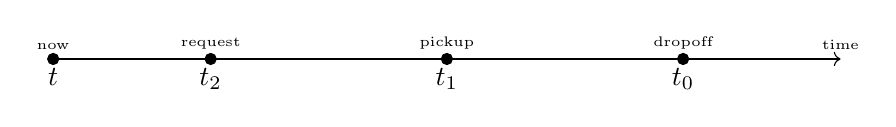
\begin{tikzpicture}
  \draw[->] (0,0) -- (10,0) node[above]{\tiny time}; % Arrow line
  \filldraw[black] (2,0) circle (2pt) node[below] {$t_2$} node[above] {\tiny request};
  \filldraw[black] (5,0) circle (2pt) node[below] {$t_1$} node[above] {\tiny pickup};
  \filldraw[black] (8,0) circle (2pt) node[below] {$t_0$} node[above] {\tiny dropoff};
  \filldraw[black] (0,0) circle (2pt) node[below] {$t$} node[above] {\tiny now};
\end{tikzpicture}
\caption{Ride progress stages: from current time, to request, pickup and dropoff. }
\label{fig:ride-time}
\end{figure}

Section~\ref{sec:pricing-main} discussed the pricing of an "On-demand" single ride, conditioned on a path, see~\eqref{eq:price} and ~\eqref{eq:predicted-price}. It is now possible to generalize the pricing method developed to different products, as in the following.
\begin{enumerate}[label={({\Alph*})}]
    \item On-demand. An instantaneous ride request to go from  $\pstart$ to $\pend$ in $\cG$,   \label{on-demand}
    \item Scheduled. A ride request to go from $\pstart$ to $\pend$ in $\cG$ at a future time $t$,  \label{scheduled}
    \item Membership. An option to request up to $R \in \ZZ$ rides within a pacified time interval, say $[0, T_R]$, $T_R \in \RR_+$, at a predetermined discounted prices, for example $10\%$. Such rides can be (but not necessarily) conditioned over fixed times and locations.   \label{membership}
\end{enumerate}

The main challenge in all scenarios \ref{on-demand}~\ref{scheduled} and~\ref{membership}, is how to properly compute an up-front prices, which is a price paid at the time of the request or membership subscription. Scenarios~\ref{on-demand},~\ref{scheduled} and~\ref{membership} are increasingly more complex. In~\ref{on-demand} current network dynamics and start/end locations are known at the pricing time, in~\ref{scheduled} only the start/end locations are known, and network dynamics can only be predicted. In~\ref{membership} no information is known at the pricing time, moreover, the ride is elective.

\textbf{For case~\ref{on-demand}:} let 
\begin{itemize}
    \item $\rbr{\pstart, \pend}$ be the two points of interest; 
    \item$ \Pi(\pstart, \pend)$ to be the set of all paths between $\pstart$ and $\pend$. 
\end{itemize}
Then following~\eqref{eq:ride-cost}, for case~\ref{on-demand}, the on-demand price guarantee at request time $t_2$ is
\[ R(t_2, t_1, t_2, \path, K) = \EE\sbr{e^{-r(t_1-t_2 +\T_\path)}R(t_0,t_1, t_2, \path, K)}=e^{-r(t_1-t_2)}\EE\sbr{e^{-r\T_\path}R(t_0,t_1, t_2, \path, K)} \]

\textbf{For case~\ref{scheduled}:}, in addition to definitions above, let, 
\begin{itemize}
    \item $t_2$ be a fixed request time;
    \item $t$ be the scheduling time.
\end{itemize}

Then the scheduled ride price guarantee at $t$ is
\begin{align}\label{eq:scheduled-price}
    \bar R(t, t_1, t_2, K) & = 
\sum_{\path_i \in \Pi\rbr{\pstart, \pend}} R(t, t_1, t_2, \path_i, K)\pi(\path_i) \\
& = \sum_{\path_i \in \Pi\rbr{\pstart, \pend}} \EE\sbr{e^{-r(t_2-t + \T_{\path_i})}R(t_0,t_1, t_2, \path, K)}\pi(\path_i) \\
 & = \sum_{\path_i \in \Pi\rbr{\pstart, \pend}} \EE\sbr{\EE \sbr{e^{-r(t_2-t) - r\T_{\path_i}}R(t_0,t_1, t_2, \path, K)\given t_2}}\pi(\path_i) \\
& = e^{-r(t_2-t)} \sum_{\path_i \in \Pi\rbr{\pstart, \pend}} \EE\sbr{e^{-r\T_{\path_i}}R(t_0,t_1, t_2, \path, K)}\pi(\path_i).
\end{align}

The pricing in~\eqref{eq:scheduled-price} occurs by averaging over all routes between $\pstart$ and $\pend$. 


\textbf{For case~\ref{membership}}, let
\begin{itemize}
    \item $M \in \NN$ be the maximum number of rides;
    \item $\rbr{\pstart, \pend} \cG$ be the pair of star and end locations, that is fixed to the membership
    \item $t=0$ be the purchase price of the membership. 
    \item $K$ is the fixed price to go from $\pstart$ to $\pend$.
\end{itemize}

Pricing this membership would be 

\begin{align}\label{eq:membership-price}
    \bar R(t, M, \pstart, \pend) & = M
    \sum_{t_2 \in [0, T_R]} 
    \sum_{\path_i \in \Pi\rbr{\pstart, \pend}} 
    R\rbr{t, t_1, t_2, \path_i, K_{\path_i}}
    \pi(t_2) \pi(\path_i), \\
    & = M \sum_{t_2 \in [0, T_R]} e^{-r\rbr{t_2 - t}}
    \sum_{\path_i \in \Pi\rbr{\pstart, \pend}} 
    R\rbr{t_2, t_1, t_2, \path_i, K}
    \pi(t_2) \pi(\path_i), \\
      & = M \sum_{t_2 \in [0, T_R]} e^{-r\rbr{t_2 - t}}
    \sum_{\path_i \in \Pi\rbr{\pstart, \pend}} 
    \EE\sbr{e^{-r\T_{\path_i}}R\rbr{t_0, t_1, t_2, \path_i, K}}
    \pi(t_2) \pi(\path_i), \\
    & = M \sum_{t_2 \in [0, T_R]} e^{-r\rbr{t_2 - t}} \bar R\rbr{t_2, t_1, t_2, K}   \pi(t_2),
\end{align}
where $\bar R$ follows~\eqref{eq:scheduled-price}.


\section{Case study} \label{sec:case-study}


\section{Discussion}

In turn, providers build complex models that attempt a sweet spot between profitability and competitiveness. Such predictive models often rely on point-estimates of travel time without accounting for travel uncertainty. Integrating of uncertainty in pricing structures proved elusive for two reasons; (a) analytical approaches are still lacking, and




\bibliographystyle{plainnat}
\bibliography{references}

\end{document}